\documentclass[12pt,a4paper]{article}
%\usepackage{ctex}
\usepackage{amsmath,amscd,amsbsy,amssymb,latexsym,url,bm,amsthm}
\usepackage{epsfig,graphicx,subfigure}
\usepackage{enumitem,balance}
\usepackage{wrapfig}
\usepackage{mathrsfs,euscript}
\usepackage[x11names,svgnames,dvipsnames]{xcolor}
\usepackage{hyperref}
\usepackage[vlined,ruled,commentsnumbered,linesnumbered]{algorithm2e}
\usepackage{listings}
\usepackage{multicol}
%\usepackage{fontspec}

\renewcommand{\listalgorithmcfname}{List of Algorithms}
\renewcommand{\algorithmcfname}{Alg.}
\newtheorem{theorem}{Theorem}
\newtheorem{lemma}[theorem]{Lemma}
\newtheorem{proposition}[theorem]{Proposition}
\newtheorem{corollary}[theorem]{Corollary}
\newtheorem{exercise}{Exercise}
\newtheorem*{solution}{Solution}
\newtheorem{definition}{Definition}
\theoremstyle{definition}


%\numberwithin{equation}{section}
%\numberwithin{figure}{section}

\renewcommand{\thefootnote}{\fnsymbol{footnote}}

\newcommand{\postscript}[2]
 {\setlength{\epsfxsize}{#2\hsize}
  \centerline{\epsfbox{#1}}}

\renewcommand{\baselinestretch}{1.0}

\setlength{\oddsidemargin}{-0.365in}
\setlength{\evensidemargin}{-0.365in}
\setlength{\topmargin}{-0.3in}
\setlength{\headheight}{0in}
\setlength{\headsep}{0in}
\setlength{\textheight}{10.1in}
\setlength{\textwidth}{7in}
\makeatletter \renewenvironment{proof}[1][Proof] {\par\pushQED{\qed}\normalfont\topsep6\p@\@plus6\p@\relax\trivlist\item[\hskip\labelsep\bfseries#1\@addpunct{.}]\ignorespaces}{\popQED\endtrivlist\@endpefalse} \makeatother
\makeatletter
\renewenvironment{solution}[1][Solution] {\par\pushQED{\qed}\normalfont\topsep6\p@\@plus6\p@\relax\trivlist\item[\hskip\labelsep\bfseries#1\@addpunct{.}]\ignorespaces}{\popQED\endtrivlist\@endpefalse} \makeatother


\definecolor{codegreen}{rgb}{0.44,0.68,0.28}
\definecolor{codegray}{rgb}{0.5,0.5,0.5}
\definecolor{codepurple}{rgb}{0.58,0,0.82}
\definecolor{backcolour}{rgb}{0.96,0.96,0.96}

\lstset{
language=C++,
frame=shadowbox,
keywordstyle = \color{blue}\bfseries,
commentstyle=\color{codegreen},
tabsize = 4,
backgroundcolor=\color{backcolour},
numbers=left,
numbersep=5pt,
breaklines=true,
emph = {int,float,double,char},emphstyle=\color{orange},
emph ={[2]const, typedef},emphstyle = {[2]\color{red}} }



\begin{document}
\noindent

%========================================================================
\noindent\framebox[\linewidth]{\shortstack[c]{
\Large{\textbf{Lab08-Graphs}}\vspace{1mm}\\
VE281 - Data Structures and Algorithms, Xiaofeng Gao, TA: Li Ma, Autumn 2019}}
%CS26019 - Algorithm Design and Analysis, Xiaofeng Gao, Autumn 2019}}
\begin{center}
%\footnotesize{\color{red}$*$ Please upload your assignment to website. Contact webmaster for any questions.}

\footnotesize{\color{blue}$*$ Name: Jin Zhejian \quad Student ID: 517370910167 \quad Email: jinzhejian@outlook.com}
\end{center}


\begin{enumerate}

\item \textbf{DAG.} Suppose that you are given a directed acyclic graph $G=(V,E)$ with real-valued edge weights and two distinct nodes $s$ and $d$. Describe an algorithm for finding a longest weighted simple path from $s$ to $d$. For example, for the graph shown in Figure 1, the longest path from node $A$ to node $C$ should be $A \rightarrow B \rightarrow F \rightarrow C$. If there is no path exists between the two nodes, your algorithm just tells so. What is the efficiency of your algorithm? (Hint: consider topological sorting on the DAG.)



\begin{figure}[htbp]
% \begin{minipage}[t]{0.5\linewidth}
% \centering
% 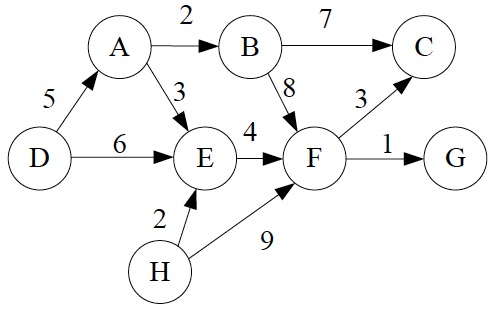
\includegraphics[scale=0.35]{Lab08-figure1.jpg}
% \caption{A weighted undirected graph.}
% \end{minipage}%
% \begin{minipage}[t]{0.5\linewidth}
\centering
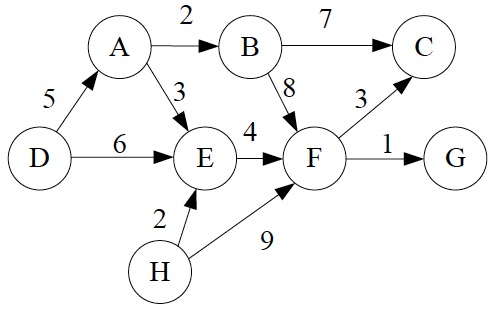
\includegraphics[scale=0.35]{Lab08-figure1.jpg}
\caption{A weighted directed graph.}
% \end{minipage}
\end{figure}


\begin{solution}
	~\\
   \textbf{My algorithm}:
   \begin{enumerate}
   	\item Initialize distance array dist[] , where every entry is negative infinite except that: dist[s] = 0, which s is the source node.
   	\item Topological sort the graph,  save the result in a stack.
   	\item
   	for every vertex u in topological order\{
   		
   	\qquad for every adjacent  vertex v of u\{
   
   \qquad \qquad if (dist[v] < dist[u] + weight(u, v))\{
   
    \qquad \qquad \qquad dist[v] = dist[u] + weight(u, v)
    
    \qquad \qquad \}
   
   \qquad \}
   
   \}
   
   \end{enumerate}
	
	\textbf{Time complexity}:
	
	For the (b) part, the time complexity of topological sorting is O(V+E). 
	
	For the (c) part, we have v nodes and total adjacent vertices is E, so we need  O(V+E). 
	
	Overall, the time complexity of this algorithm is O(V+E).
	
	\textbf{Implementation and outcome}:
	
	 The DAG.cpp implementation of my algorithm is shown in the Appendix part.

	The following is the output of my cpp code, in which I use number instead of alphabet for convenience (A = 0, B = 1, C = 2, D = 3, E = 4, F = 5, G = 6, H = 7):
	 \begin{lstlisting}
	Following are longest distances from s 0 to d 2 
	Path is 0 1 5 2
	distance is 13 
	\end{lstlisting}
	
\end{solution}



\item \textbf{ShortestPath.} Suppose that you are given a directed graph $G=(V,E)$ on which each edge $(u,v) \in E$ has an associated value $r(u,v)$, which is a real number in the range $0 \leq r(u,v) \leq 1$ that represents the reliability of a communication channel from vertex $u$ to vertex $v$. We interpret $r(u,v)$ as the probability that the channel from $u$ to $v$ will not fail, and we assume that these probabilities are independent. Give an efficient algorithm to find the most reliable path between two given vertices.

\begin{solution}
	~\\
	My solution is similar to the solution in the first problem.
	
\textbf{My algorithm}:
   \begin{enumerate}
	\item Initialize distance array dist[] , where every entry is negative infinite except that: dist[s] = 1, which s is the source vertice.
	\item Topological sort the graph,  save the result in a stack.
	\item
	for every vertex u in topological order\{
	
	\qquad for every adjacent  vertex v of u\{
	
	\qquad \qquad if (dist[v] < dist[u] $\cdot$ r(u, v))\{
	
	\qquad \qquad \qquad dist[v] = dist[u] $\cdot $ r(u, v)
	
	\qquad \qquad \qquad if (v is the end vertice) \{
	
	\qquad \qquad \qquad \qquad add u to the path of source to end vertice
	
	\qquad \qquad \qquad \}
	
	\qquad \qquad \}
	
	\qquad \}
	
	\}
	
	

\end{enumerate}

\textbf{Time complexity}:

Still O(V+E). As explained in the first problem.

\end{solution}

\item \textbf{GraphSearch.} Let $G=(V,E)$ be a connected, undirected graph. Give an $O(|V|+|E|)$-time algorithm to compute a path in $G$ that traverses each edge in $E$ \textbf{exactly once in each direction}. For example, for the graph shown in Figure 2, one path satisfying the requirement is
$$A \rightarrow B \rightarrow C \rightarrow D \rightarrow C \rightarrow A \rightarrow C \rightarrow B \rightarrow A$$
Note that in the above path, each edge is visited exactly once in each direction.

\begin{figure}[h]
 \centering
 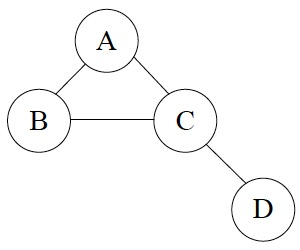
\includegraphics[scale=0.35]{Lab08-figure2.jpg}
 \caption{A undirected graph.}
\end{figure}

\begin{solution}
	We can make a little change to  DFS:

	\begin{algorithm}[H]
	\caption{DFS\_change($u$)} \label{DFS}

	VISITED(u) = TRUE;
	
	\ForEach{v $\in$ adj(u)}{
	
	\If{!VISITED(v)}{
	
	set depth[v] = depth[u] + 1
	
	traverse edge $u \rightarrow v$;
	
	DFS\_change($v$);
	
	traverse edge $u \rightarrow v$;
	}

 \ElseIf{depth[v] > depth[u]}{
 	
			traverse edge $u \rightarrow v$;
			
			traverse edge $u \rightarrow v$;
	}
	
	}

\end{algorithm}
\end{solution}

\end{enumerate}



\newpage
\noindent{\large \textbf{Appendix}}

\noindent (1) DAG.cpp
 \begin{lstlisting}
#include <iostream>
#include <limits.h>
#include <list>
#include <stack>
#define NINF INT_MIN
using namespace std;

class AdjListNode {
int v;
int weight;

public:
AdjListNode(int _v, int _w){
v = _v;
weight = _w;
}
int getV() { return v; }
int getWeight() { return weight; }
};

class Graph {
// No. of vertices
int V;
// Pointer to an array containing adjacency lists
list<AdjListNode>* adj;
void topologicalSortUtil(int v, bool visited[], stack<int>& Stack);
public:
Graph(int V); // Constructor
~Graph(); // Destructor
void addEdge(int u, int v, int weight);
// Finds longest distances from given source vertex
void longestPath(int s, int d);
};

Graph::Graph(int V) // Constructor
{
this->V = V;
adj = new list<AdjListNode>[V];
}

Graph::~Graph() // Destructor
{
delete [] adj;
}

void Graph::addEdge(int u, int v, int weight)
{
AdjListNode node(v, weight);
adj[u].push_back(node);
}

void Graph::topologicalSortUtil(int v, bool visited[], stack<int>& Stack)
{
// Mark the current node as visited
visited[v] = true;

// Recur for all the vertices adjacent to this vertex
list<AdjListNode>::iterator i;
for (i = adj[v].begin(); i != adj[v].end(); ++i) {
AdjListNode node = *i;
if (!visited[node.getV()])
topologicalSortUtil(node.getV(), visited, Stack);
}

// Push current vertex to stack which stores topological sort
Stack.push(v);
}

void Graph::longestPath(int s, int d)
{
stack<int> Stack;
int dist[V];

bool* visited = new bool[V];
for (int i = 0; i < V; i++) {
visited[i] = false;
}

// Call the recursive helper function to store Topological
// Sort starting from all vertices one by one
for (int i = 0; i < V; i++) {
if (!visited[i]) {
topologicalSortUtil(i, visited, Stack);
}
}

// Initialize distances to all vertices as infinite and
// distance to source as 0
for (int i = 0; i < V; i++) {
dist[i] = NINF;
}

dist[s] = 0;

// Process vertices in topological order
cout << "Path is "  << s << " ";
while (!Stack.empty()) {
// Get the next vertex from topological order
int u = Stack.top();
Stack.pop();

// Update distances of all adjacent vertices
list<AdjListNode>::iterator i;
if (dist[u] != NINF) {
for (i = adj[u].begin(); i != adj[u].end(); ++i) {
if (dist[i->getV()] < dist[u] + i->getWeight()) {
dist[i->getV()] = dist[u] + i->getWeight();
}
if (i->getV() == d) {cout <<  u <<  " " ;}
}
}
}

// Print the calculated longest distances
//    for (int i = 0; i < V; i++) {
//        (dist[i] == NINF) ? cout << "INF " : cout << dist[i] << " ";
//    }
cout << d <<  endl;
(dist[d] == NINF) ? cout << "distance is INF " : cout << "distance is " << dist[d]  << " ";

delete [] visited;
}

// Driver program to test above functions
int main()
{
int A = 0, B = 1, C = 2, D = 3, E = 4, F = 5, G = 6, H = 7;
Graph g(8);
g.addEdge(A,B,2);
g.addEdge(A,E,3);
g.addEdge(B,C,7);
g.addEdge(B,F,8);
g.addEdge(D,A,5);
g.addEdge(D,E,6);
g.addEdge(E,F,4);
g.addEdge(F,C,3);
g.addEdge(F,G,1);
g.addEdge(H,E,2);
g.addEdge(H,G,9);

int s = 0;
int d= 2;
cout << "Following are longest distances from s "
<< s  << " to d " << d << " \n";
g.longestPath(s,d);
return 0;
}	
\end{lstlisting}


%========================================================================
\end{document}
